\documentclass[11pt]{beamer}
\usetheme{default}
\usecolortheme{beaver}
\usepackage{fancyvrb}
\usepackage[utf8]{inputenc}
\usepackage{pmboxdraw}
\usepackage[english]{babel}
\usepackage{amsmath}
\usepackage{amsfonts}
\usepackage{amssymb}
\usepackage{listings}
\author{Mattia Bacarella - 928345\\
		Francesco Corda - 920212\\
		Davide Damato - 920616\\
		Luciano Franchin - 921093\\
		Luca Massini - 945027}
\title{Pricing and Advertising}
\subtitle{Project for the Data Intelligence Application Class\\
		PoliMi 2019-2020}
		
\usepackage{xcolor}

\definecolor{codegreen}{rgb}{0,0.6,0}
\definecolor{codegray}{rgb}{0.5,0.5,0.5}
\definecolor{codepurple}{rgb}{0.58,0,0.82}
\definecolor{backcolour}{rgb}{0.95,0.95,0.92}

\lstdefinestyle{mystyle}{
	language = Python,
    backgroundcolor=\color{backcolour},   
    commentstyle=\color{codegreen},
    keywordstyle=\color{magenta},
    numberstyle=\tiny\color{codegray},
    stringstyle=\color{codepurple},
    basicstyle=\ttfamily\footnotesize,
    breakatwhitespace=false,         
    breaklines=true,                 
    captionpos=b,                    
    keepspaces=true,                 
    numbers=left,                    
    numbersep=5pt,                  
    showspaces=false,                
    showstringspaces=false,
    showtabs=false,                  
    tabsize=2
}

\lstset{style=mystyle}

\begin{document}

\begin{frame}
\titlepage
\end{frame}

%\begin{frame}
%\tableofcontents
%\end{frame}

\begin{frame}{Objective of the Project}
\textit{The goal is to model a scenario in which a seller exploits advertising tools to attract more and more users to its website, thus increasing the number of possible buyers. The seller needs to learn simultaneously the conversion rate and the number of users the advertising tools can attract.}
\end{frame}

\begin{frame}[fragile]{Project Structure}
\begin{itemize}
\item Repository: \url{https://github.com/francescocorda/dia-project}
\item Structure:
\begin{verbatim}
dia_project
 ├── assignment_2
 ├── assignment_3
 ├── assignment_4
 ├── assignment_5
 ├── assignment_6
 ├── assignment_7
 ├── data
 └── utils
\end{verbatim}
\item The project is organized in modules, one for each assignment. To execute the code and reproduce our results, run the file assignment\_x.py in each module.
\end{itemize}
\end{frame}

\begin{frame}{Project Roadmap}
After the definition of the working environment, the project can be divided in three main sections:
\begin{itemize}
\item a first part dedicated to advertising the product, with the goal of maximizing the traffic (expressed as number of clicks) directed to our web page
\item a second part dedicated to the pricing, with the goal of finding the optimal selling point to obtain the highest revenue
\item a third part in which the actions are combined, the algorithm learns simultaneously to advertise and sell
\end{itemize}
\begin{figure}[hbtp]
\centering
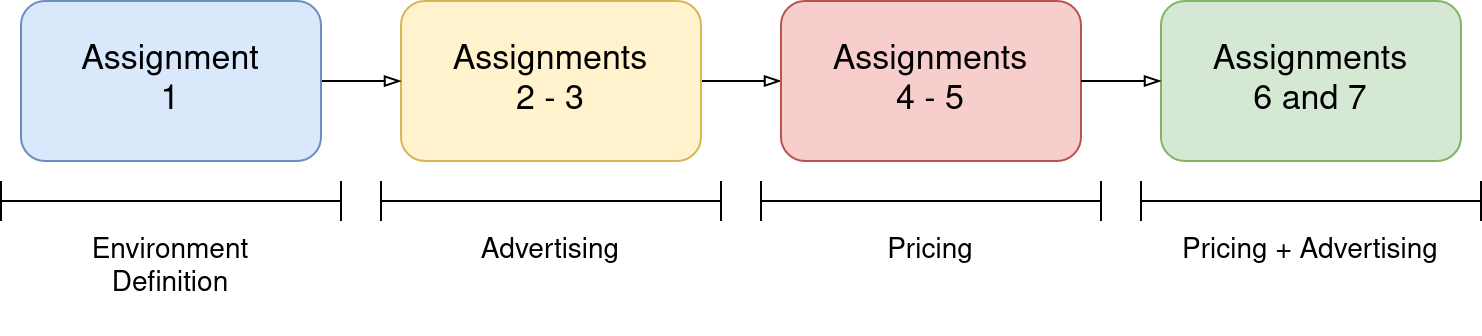
\includegraphics[width=\textwidth]{images/roadmap.png}
\end{figure}

\end{frame}

\begin{frame}{Assignment 1}
\textit{Imagine one product to sell:
\begin{itemize}
\item three classes of users, where, for every user, we can observe the values of two binary features (feel free to choose the features and their domains);
\item the conversion rate curve of each class of users;
\item three subcampaigns, each with a different ad, to advertise the product, and each targeting a different class of users;
\item there are three abrupt phases;
\item for every abrupt phase and for every subcampaign, the probability distribution over the daily number of clicks for every value of budget allocated to that subcampaign.
\end{itemize}}
\end{frame}

\begin{frame}{Assignment 1 - The Product}
We decided to analyze the pricing and the advertising of a \textbf{gym membership}, a product that presents the following properties:
\begin{itemize}
\item it's a well-known and established item, used by a vast and diversified population of users
\item it's a highly customizable product, that allows for different advertising campaigns and price offers for different classes of users
\item it's strongly affected by seasonality during the year
\end{itemize}
\end{frame}

\begin{frame}{Assignment 1 - Users}
The users are characterized with a set of 2 binary features, namely:
\begin{itemize}
\item Age = \{Under 40, Over 40\}
\item Fitness Level = \{Novice, Experienced\}
\end{itemize}
We decided to focus on the following 3 classes generated by the features:
\begin{itemize}
\item (Under 40, Novice)
\item (Under 40, Experienced)
\item (Over 40, Experienced)
\end{itemize}
We excluded the class of (Over 40, Novice) users because of the online nature of our advertising campaign: an adult person which is not already interested in fitness is less likely to look on the internet for arguments related to our campaign.
\end{frame}

\begin{frame}{Assignment 1 - (Under 40, Novice) class}
\begin{figure}[hbtp]
\centering
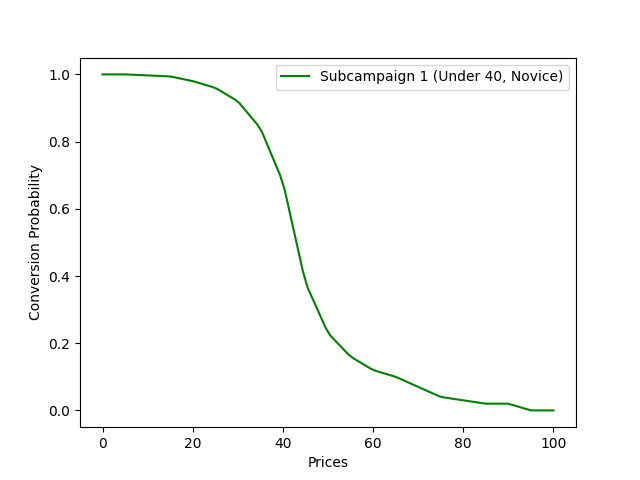
\includegraphics[width=0.8\textwidth]{images/demand_curve_1.png}
\caption{}
\end{figure}
\end{frame}

\begin{frame}{Assignment 1 - (Under 40, Experienced) class}
\begin{figure}[hbtp]
\centering
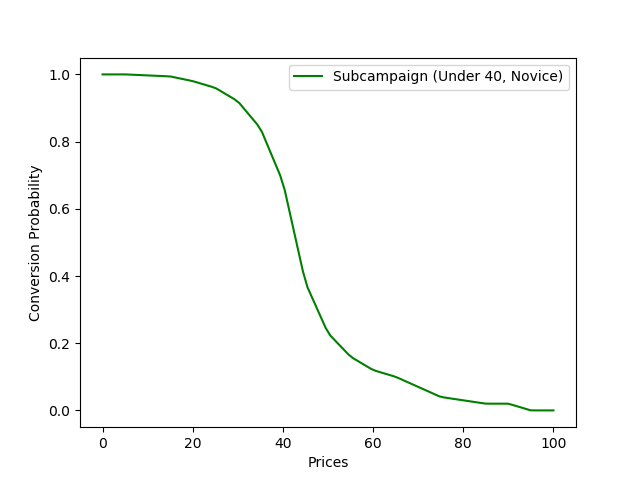
\includegraphics[width=0.8\textwidth]{images/demand_curve_2.png}
\caption{}
\end{figure}
\end{frame}

\begin{frame}{Assignment 1 - (Over 40, Experienced) class}
\begin{figure}[hbtp]
\centering
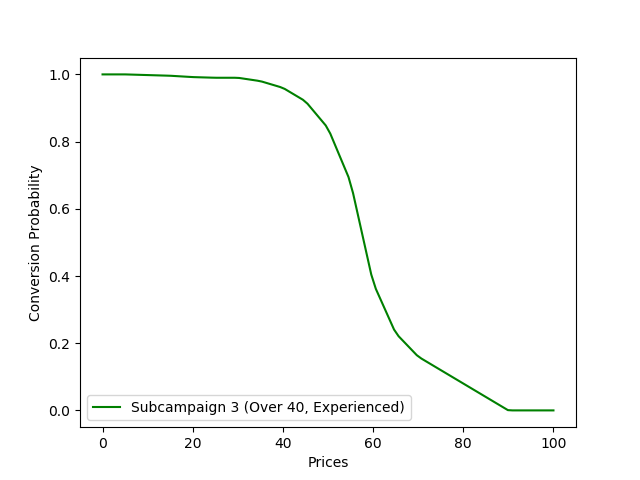
\includegraphics[width=0.8\textwidth]{images/demand_curve_3.png}
\caption{}
\end{figure}
\end{frame}

\begin{frame}{Assignment 1 - Subcampaign 1}
\begin{figure}[hbtp]
\centering
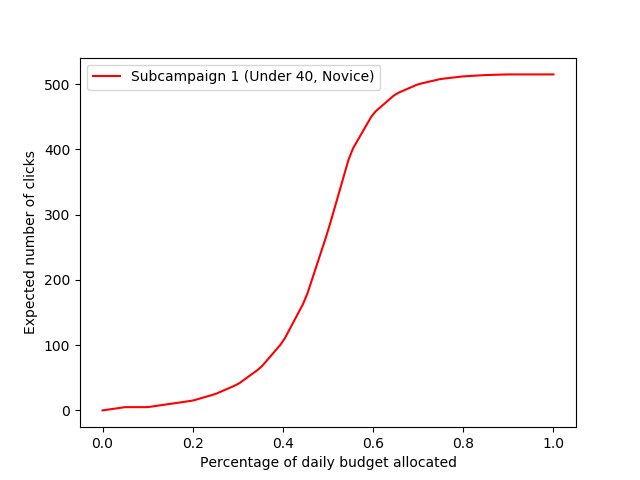
\includegraphics[width=0.8\textwidth]{images/subcampaign_1.png}
\caption{}
\end{figure}
\end{frame}

\begin{frame}{Assignment 1 - Subcampaign 2}
\begin{figure}[hbtp]
\centering
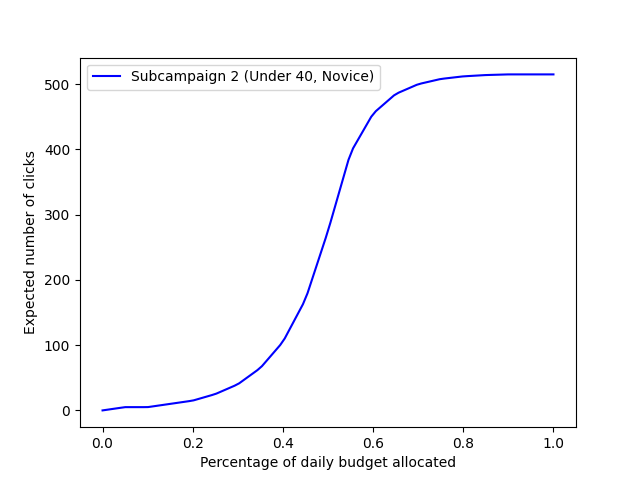
\includegraphics[width=0.8\textwidth]{images/subcampaign_2.png}
\caption{}
\end{figure}
\end{frame}

\begin{frame}{Assignment 1 - Subcampaign 3}
\begin{figure}[hbtp]
\centering
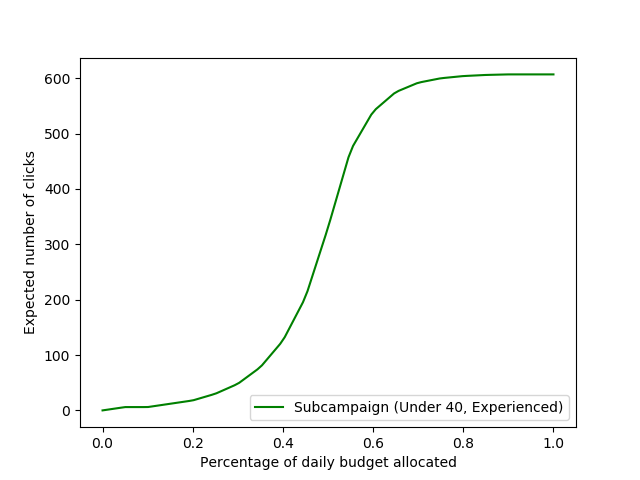
\includegraphics[width=0.8\textwidth]{images/subcampaign_3.png}
\caption{}
\end{figure}
\end{frame}

\begin{frame}{Assignment 1 - Abrupt Phases}
We identified 3 abrupt phases influenced by the seasonality that characterizes gym subscriptions during a year:
\begin{itemize}
\item [1.] [January-April], the ``New Year's Resolutions" phase
\item [2.] [May-August], the ``Swimsuit Season" phase
\item [3.] [September-December], the ``Back to Normal" phase
\end{itemize}
\vspace{\baselineskip}
Each period has the same length of 4 months and is denoted by almost-stationary behaviors of the users for its duration. 
\end{frame} 

\begin{frame}{Assignment 1 - Subcampaign 1, Abrupt Phases}
\begin{figure}[hbtp]
\centering
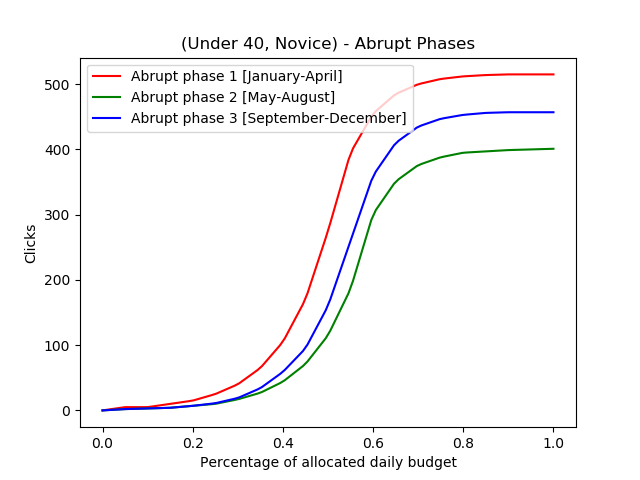
\includegraphics[width=0.8\textwidth]{images/subcampaign_1_abrupt_phases.png}
\caption{}
\end{figure}
\end{frame}

\begin{frame}{Assignment 1 - Subcampaign 2, Abrupt Phases}
\begin{figure}[hbtp]
\centering
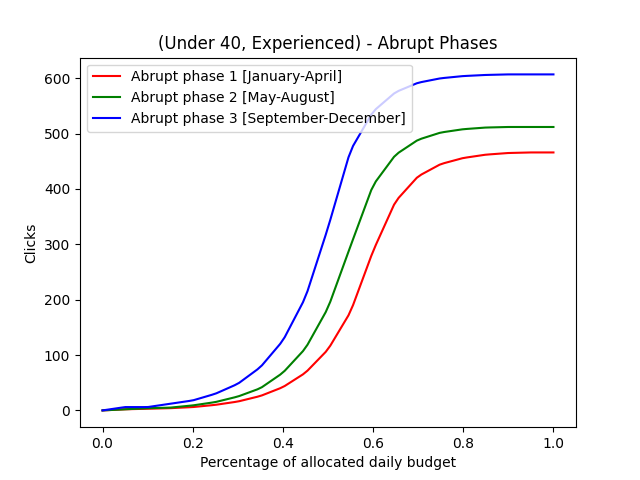
\includegraphics[width=0.8\textwidth]{images/subcampaign_2_abrupt_phases.png}
\caption{}
\end{figure}
\end{frame}

\begin{frame}{Assignment 1 - Subcampaign 3, Abrupt Phases}
\begin{figure}[hbtp]
\centering
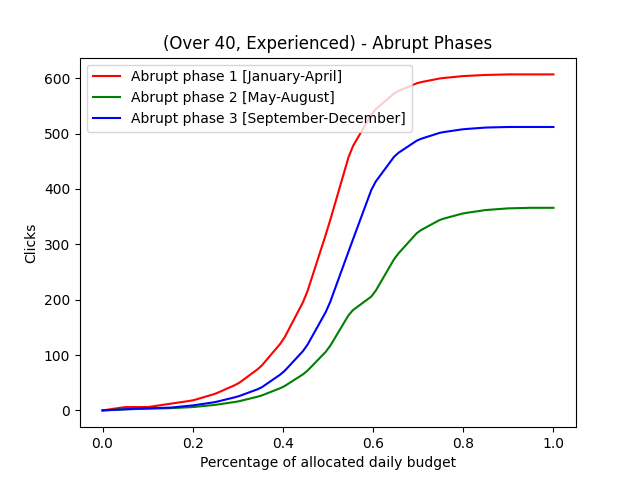
\includegraphics[width=0.8\textwidth]{images/subcampaign_3_abrupt_phases.png}
\caption{}
\end{figure}
\end{frame}

\begin{frame}{Assignment 2}
\textit{Design a combinatorial bandit algorithm to optimize the budget allocation over the three subcampaigns to maximize the total number of clicks when, for simplicity, there is only one phase. Plot the cumulative regret.}
\end{frame}

\begin{frame}[fragile]{Assignment 2 - Pseudocode}
\begin{lstlisting}
initialize click envs
for exp in n_experiments:
  initialize gp-ts learners
  for t in time_horizon:
    draw samples for each subcampaign
    find super-arm by solving knapsack problem
    pull arms given by super-arm
    update gp-ts learners
calculate clairvoyant value
plot rewards and regrets
\end{lstlisting}
\end{frame}

\begin{frame}{Assignment 2 -  Cumulative Regret}
\begin{figure}[hbtp]
\centering
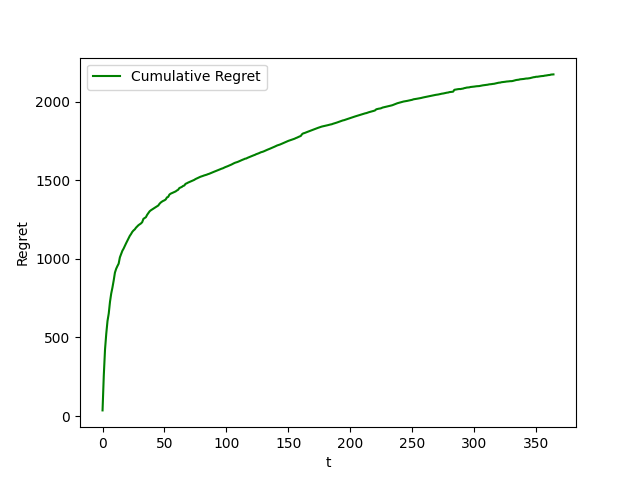
\includegraphics[width=0.8\textwidth]{images/assignment_2_cum_regret.png}
\caption{}
\end{figure}
\end{frame}

\begin{frame}{Assignment 2 - Regret}
\begin{figure}[hbtp]
\centering
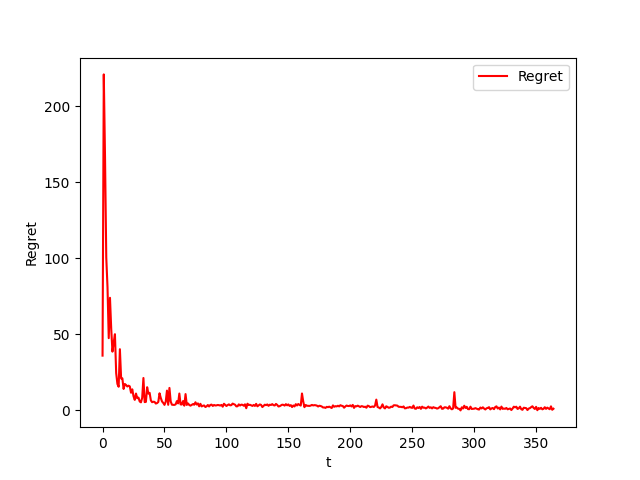
\includegraphics[width=0.8\textwidth]{images/assignment_2_regret.png}
\caption{}
\end{figure}
\end{frame}

\begin{frame}{Assignment 3}
\textit{Design a sliding-window combinatorial bandit algorithm for the case, instead, in which there are the three phases aforementioned. Plot the cumulative regret and compare it with the cumulative regret that a non-sliding-window algorithm would obtain.}
\end{frame}

\begin{frame}[fragile]{Assignment 3 - Pseudocode}
\begin{lstlisting}
initialize click envs
for exp in n_experiments:
  initialize gp-ts and gp-ts-sw learners 
  for t in time_horizon:
  	if abprupt_phase is changed:
  		reset memory of the learners
    draw samples for each subcampaign
    find super-arm by solving knapsack problem
    pull arms given by super-arm
    update gp-ts and gp-ts-sw learners
calculate clairvoyant value
plot rewards and regrets for the 2 learners
\end{lstlisting}
\end{frame}

\begin{frame}{Assignment 3 -  Cumulative Regret}
\begin{figure}[hbtp]
\centering
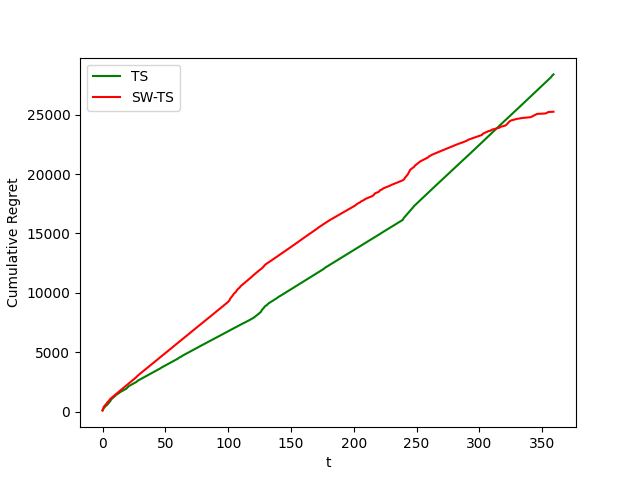
\includegraphics[width=0.8\textwidth]{images/assignment_3_cum_regret.png}
\caption{}
\end{figure}
\end{frame}

\begin{frame}{Assignment 3 - Rewards}
\begin{figure}[hbtp]
\centering
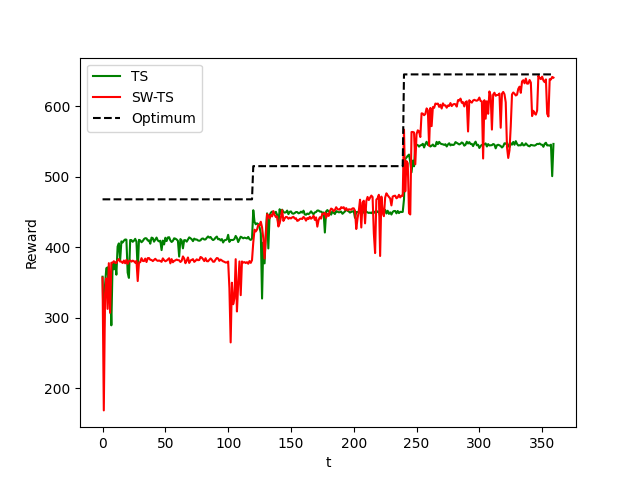
\includegraphics[width=0.8\textwidth]{images/assignment_3_reward.png}
\caption{}
\end{figure}
\end{frame}

\begin{frame}{Assignment 4}
\textit{Design a learning algorithm for pricing when the users that will buy the product are those that have clicked on the ads. Assume that the allocation of the budget over the three subcampaigns is fixed and there is only one phase (make this assumption also in the next steps). Plot the cumulative regret.}
\end{frame}

\begin{frame}[fragile]{Assignment 4 - Pseudocode}
\begin{lstlisting}
initialize pricing envs
for exp in n_experiments:
  initialize ts and greedy learners 
  for t in time_horizon:
    draw samples for each subcampaign (ts learner)
    update ts learner
    draw samples for each subcampaign (greedy learner)
    update greedy learner
calculate clairvoyant value
plot rewards and regrets for the 2 learners
\end{lstlisting}
\end{frame}

\begin{frame}{Assignment 4 - Regrets}
\begin{figure}[hbtp]
\centering
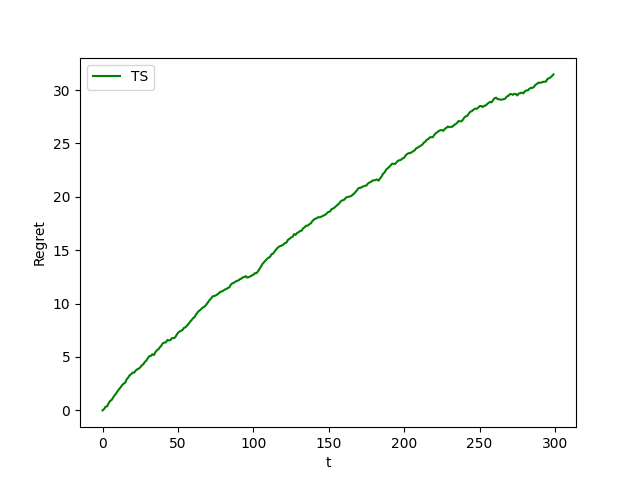
\includegraphics[width=0.8\textwidth]{images/assignment_4_regrets.png}
\caption{}
\end{figure}
\end{frame}

\begin{frame}{Assignment 5}
\textit{Design and run a context generation algorithm for the pricing when the budget allocated to each single subcampaign is fixed. At the end of every week, use the collected data to generate contexts and then use these contexts for the following week. Plot the cumulative regret as time increases. In the next steps, do not use the generated contexts, but use all the data together.}
\end{frame}

\begin{frame}[fragile]{Assignment 5 - Pseudocode}
\begin{lstlisting}
initialize pricing envs
for exp in n_experiments:
  initialize context generator 
  for t in time_horizon:
    if week is ended:
      generate new contexts (greedy approach)
    for context in n_contexts:
      run ts algorithm
calculate clairvoyant value
plot rewards and regrets
\end{lstlisting}
\end{frame}

\begin{frame}{Assignment 5 - Cumulative Regret}
\begin{figure}[hbtp]
\centering
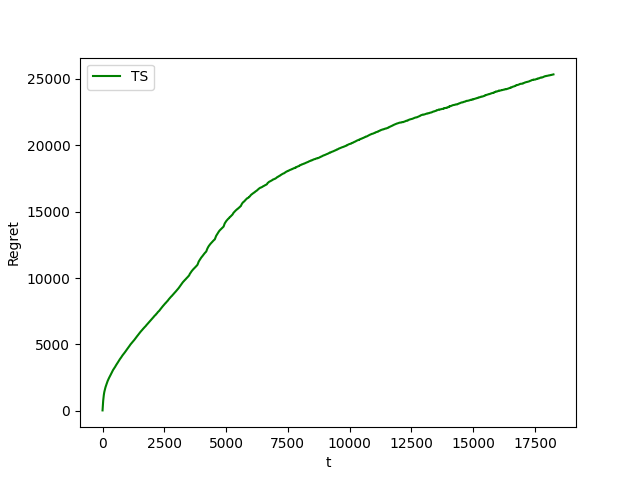
\includegraphics[width=0.8\textwidth]{images/assignment_5_cum_regret.png}
\caption{}
\end{figure}
\end{frame}

\begin{frame}{Assignment 5 - Rewards}
\begin{figure}[hbtp]
\centering
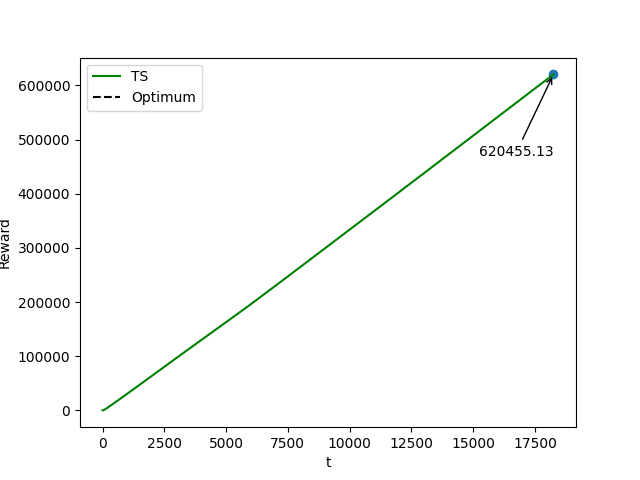
\includegraphics[width=0.8\textwidth]{images/assignment_5_reward.png}
\caption{}
\end{figure}
\end{frame}

\begin{frame}{Assignment 6}
\textit{Design an optimization algorithm combining the allocation of budget and the pricing when the seller a priori knows that every subcampaign is associated with a different context and charges a different price for every context. Suggestion: the value per click to use in the knapsack-like problem depends on the pricing, that depends on the number of users of a specific class interested in buying the product. Notice that the two problems, namely, pricing and advertising, can be decomposed since each subcampaign targets a single class of users, thus allowing the computation of the value per click of a campaign only on the basis of the number of clicks generated by that subcampaign. Plot the cumulative regret when the algorithm learns both the conversion rate curves and the performance of the advertising subcampaigns.}
\end{frame}

\begin{frame}[fragile]{Assignment 6 - Pseudocode}
\begin{lstlisting}
initialize pricing and click envs
for exp in n_experiments:
	initialize ts and gp-ts learners 
	for t in time_horizon:
		for s in subcampaign:
			draw a (price, conversion_rate) sample with ts		learner
			get return from the pricing env, given the price
			update ts learner
			draw click samples with gp-ts learner
			weight the clicks with price and conversion_rate	previously selected by the ts learner
		find super-arm by solving knapsack problem
		get revenues = clicks * price * conversion_rate from the click envs by pulling the super-arm
		update gp-ts learners 
calculate clairvoyant value
plot rewards and regrets
\end{lstlisting}
\end{frame}

\begin{frame}{Assignment 6 - Cumulative Regret}
\begin{figure}[hbtp]
\centering
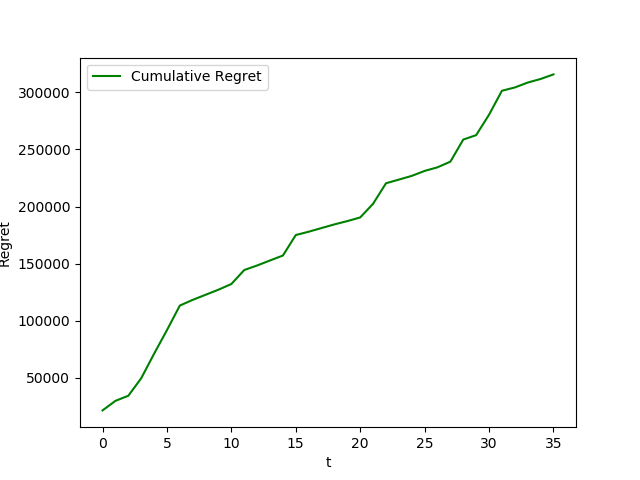
\includegraphics[width=0.8\textwidth]{images/assignment_6_cum_regret.png}
\caption{}
\end{figure}
\end{frame}

\begin{frame}{Assignment 6 - Regret}
\begin{figure}[hbtp]
\centering
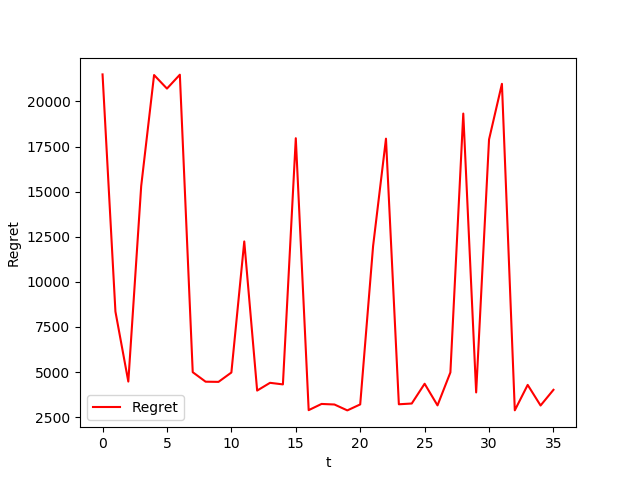
\includegraphics[width=0.8\textwidth]{images/assignment_6_regret.png}
\caption{}
\end{figure}
\end{frame}

\begin{frame}{Assignment 7}
\textit{Do the same of Step 6 under the constraint that the seller charges a unique price to all the classes of users. Suggestion: for every possible price, fix this price and repeat the algorithm used in Step 6. Plot the cumulative regret when the algorithm learns both the conversion rate curves and the performance of the advertising subcampaigns.}
\end{frame}

\begin{frame}[fragile]{Assignment 7 - Pseudocode}
\begin{lstlisting}
initialize pricing and click envs
for exp in n_experiments:
	for price in n_prices:
		initialize ts and gp-ts learners 
		for t in time_horizon:
			for s in subcampaign:
				select current price and conversion_rate 
				get return from the pricing env, given the				price
				update ts learner
				draw click samples with gp-ts learner
				weight the clicks with price and                   conversion_rate previously selected
			find super-arm by solving knapsack problem
			collect revenues = = clicks * price *             conversion_rate from the click envs by pulling    the super-arm
			update gp-ts learners 
calculate clairvoyant value
plot rewards and regrets
\end{lstlisting}
\end{frame}

\begin{frame}{Assignment 7 - Regrets}
TODO
\end{frame}

\begin{frame}{Assignment 7 - Rewards}
TODO
\end{frame}

\end{document}